\documentclass[final]{fhnwreport}         %[mode] = draft or final
\input{fhnwheader}                        %loads all packages, definitions and settings	

%%%%% Bibliographie entweder im IEEE- oder im APA-Stil:
\usepackage[style=ieee,urldate=comp,backend=biber]{biblatex}
% \usepackage[style=apa,urldate=comp,backend=biber]{biblatex}
%%%%%
\addbibresource{literature/beispiel_bib.bib}
											
\title{Steuerung für den Alexandrit-Femtosekunden Laser}  %Project Title
\author{P6 Arbeit oder Bachelor Thesis}    %Document Type => Technical Report, ...
\date{Windisch, März 2024}               %Place and Date

\begin{document}

\pagenumbering{roman}	

%%---TITLEPAGE---------------------------------------------------------------------------
\selectlanguage{ngerman}                  %ngerman or english
\maketitle

\vfill

\begin{figure}[H]
\centering
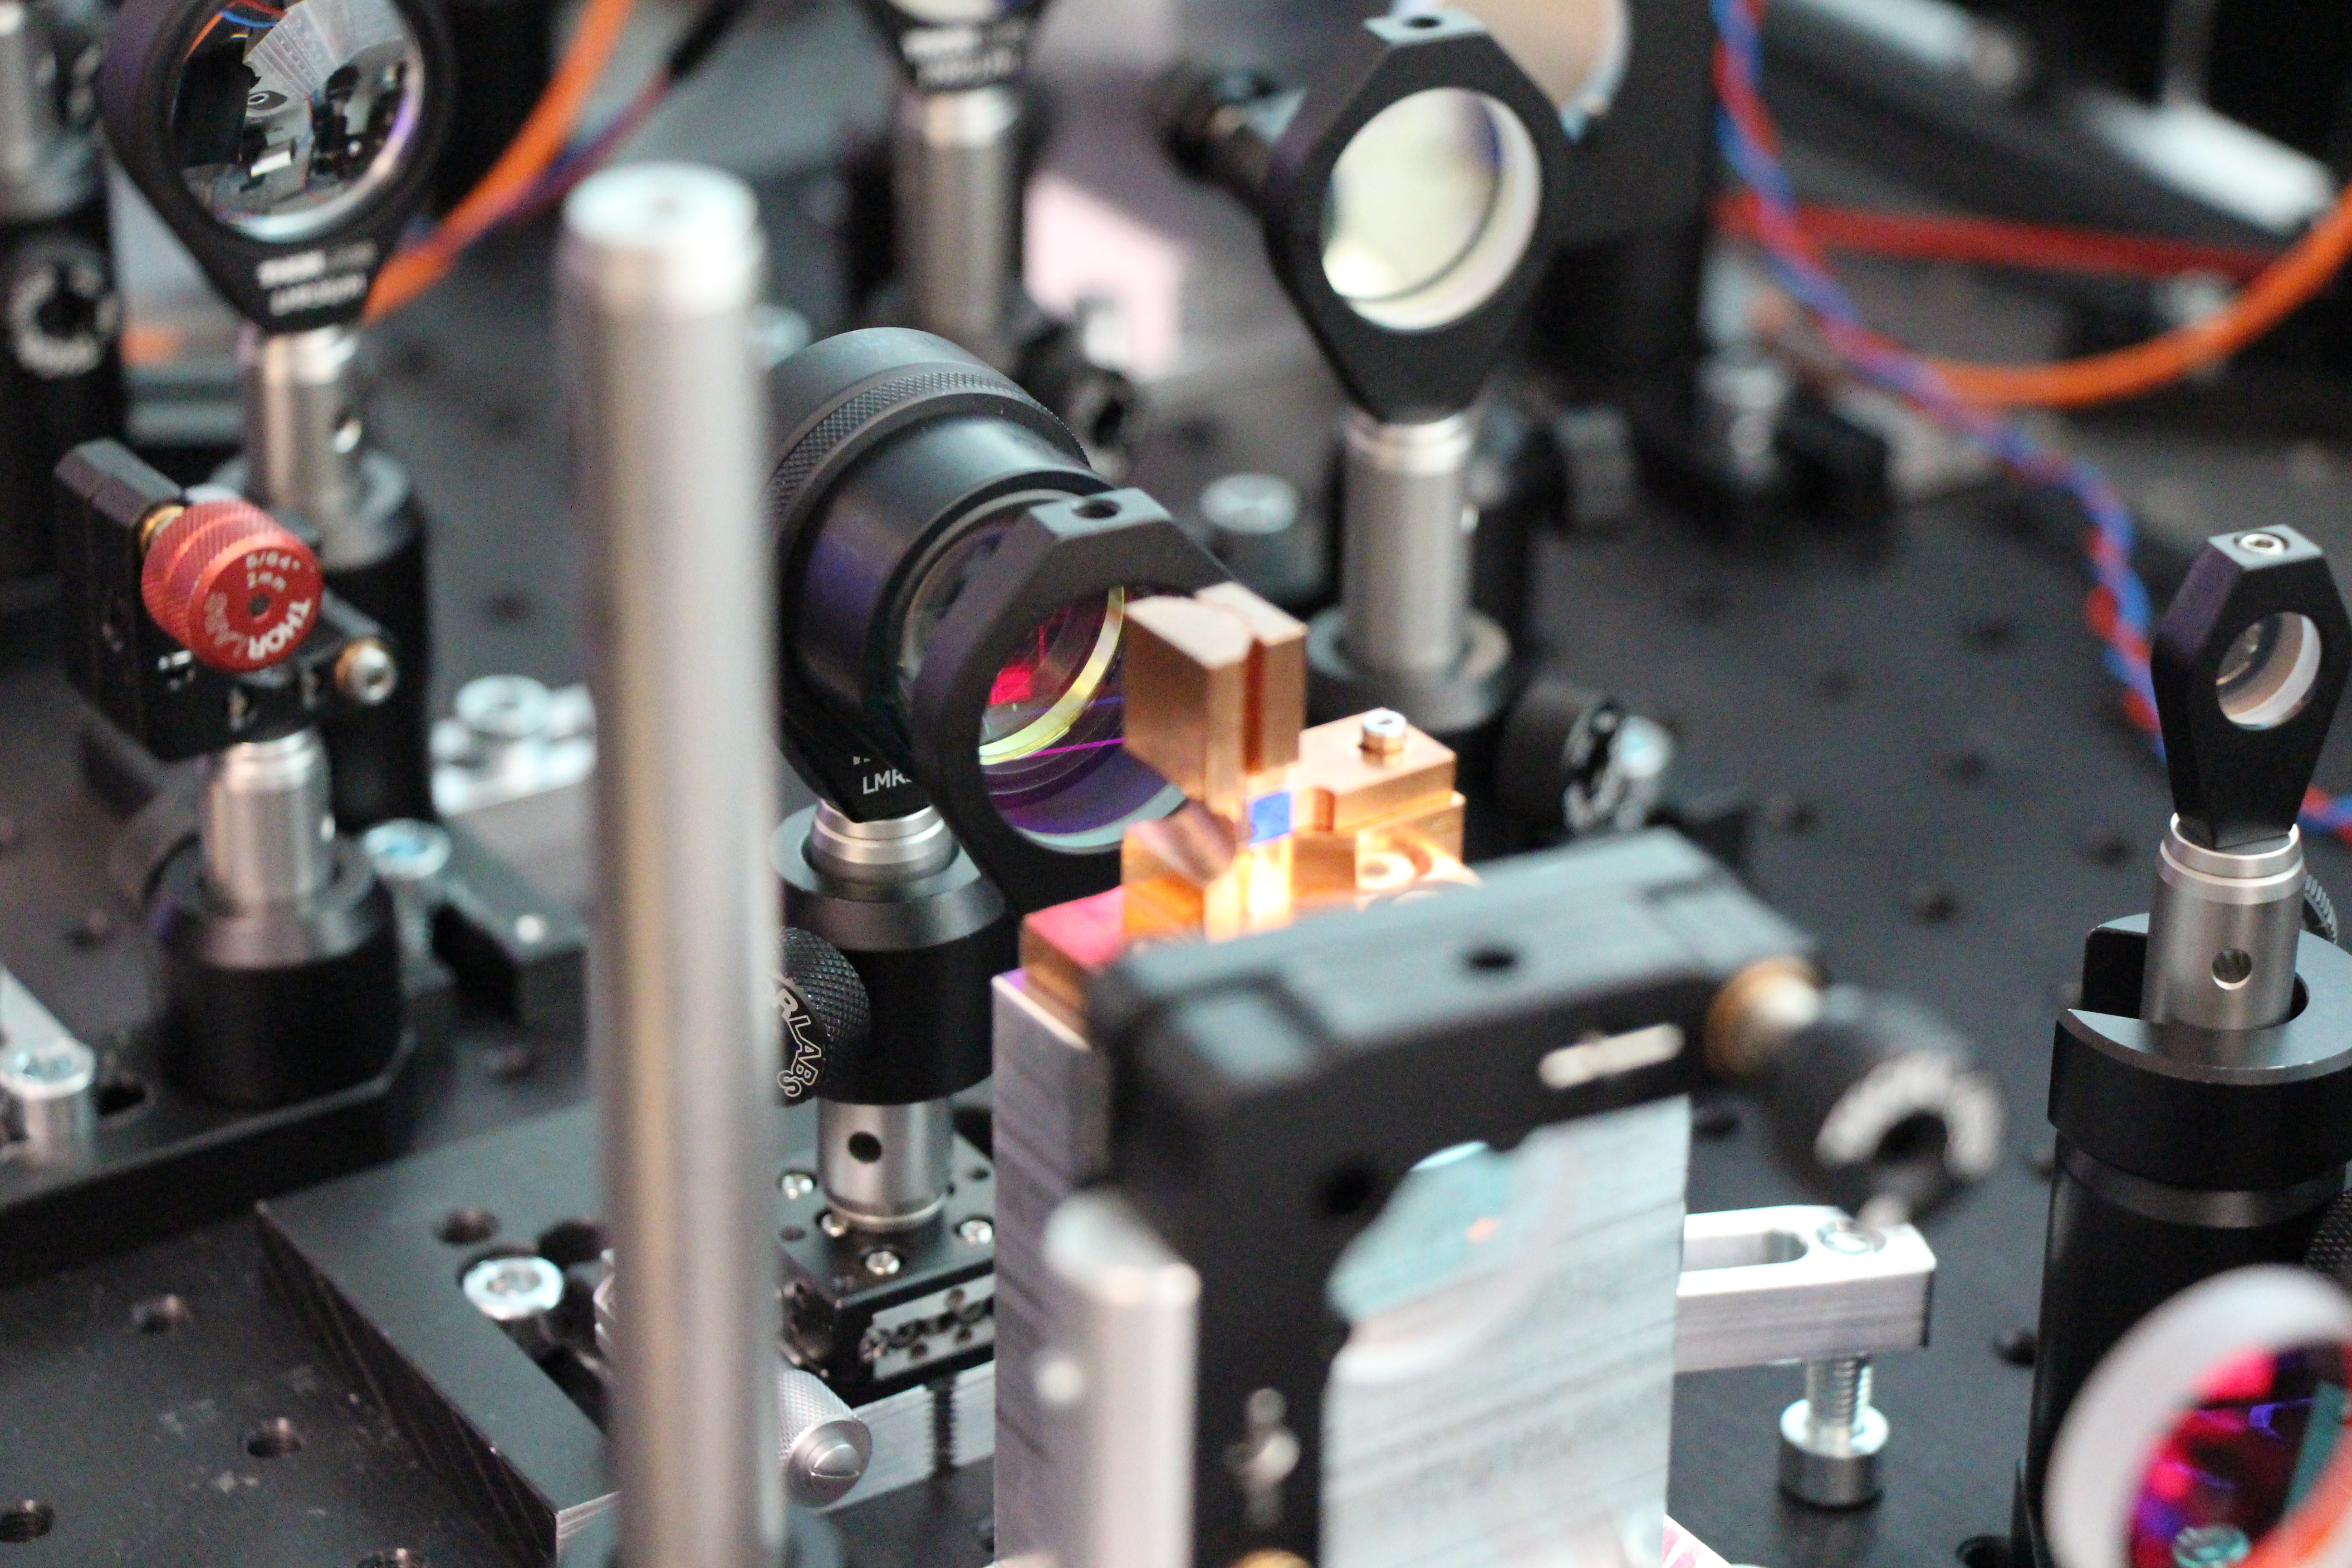
\includegraphics[width=\linewidth]{98_images/IMG_5440.JPG}
\end{figure}

\vfill

\begin{tabular}{@{}p{5cm} l}
Student&            Leroy Harreh\\[2ex]
Betreuer&           Bojan Resan\\[2ex]  % Experte
Ansprechpartner&    Tobias Grätzer\\[2ex]
Experte&            Roger Wüst\\[2ex]  % Auftraggeber
&\\
&\\
\multicolumn{2}{@{}l}{Fachhochschule Nordwestschweiz, Hochschule für Technik}
\end{tabular}

\vspace*{4ex}
% Beispiel für Logo Industriepartner
% \begin{tikzpicture}[remember picture,overlay,every node/.style={anchor=north east}]
  %\node at (current page.north east) [xshift=-1cm, yshift=-0.5cm] {\includegraphics[width=4cm]{stoica-ionela-CoNsEK5iHug-unsplash.png}};
  % Photo by Stoica Ionela on Unsplash
% \end{tikzpicture}

\clearpage

%%---ABSTRACT----------------------------------------------------------------------------
\selectlanguage{ngerman}				%ngerman or english
\thispagestyle{empty}
\section*{Abstract}
% \lipsum[1]
*In einem Abstract "Key-words" einbauen

in einem mgt summary gibt es Kapitel wohingegen das Abstract nur ein Paragraph ist

\vspace{2ex}

\textbf{Keywords:}

tic, tac

\clearpage

\section*{Danksagungen}
An dieser Stelle möchte ich mich bei all den jenigen bedanken, die mich in dieser Bachelorarbeit Betreut und Unterstützt haben.

Als erstes möchte ich mich bei Prof. Dr. Bojan Resan für das bereit gestellte Wissen, die Betreuung, die konstruktive Kritik und hilfreichen Anregungen an meiner Arbeit bedanken.\\

Zusätzlich möchte ich mich für die Unterstützung weiteren Betreuenden Personen danken, ohne die diese Projektarbeit nicht durchführbar gewesen wäre.\\ Bei Tobias Grätzer für die Einführung am Alexandirt-Laser im Labor und der Lektüre und dem Material bezüglich Lasertechnik von denen ich sehr viel profitieren konnte.

Daneben geht mein Dank an Romain Caretto, Philip Burger und Daniel Hug, welche mir Komponenten und Erfahrungen zur Verfügung gestellt haben, damit ich meine Steuerung auf ihre Funktion testen konnte.\\

Zum Schluss möchte ich mich bei meinem Arbeitskollegen Marko Obradovic für den Review meines Programmcodes und den Verbesserungsvorschlägen dessen bedanken.
\\\\
Leroy Harreh\\
Basel, März 2024



%%---TABLE OF CONTENTS-------------------------------------------------------------------	
\selectlanguage{ngerman}				%ngerman or english
\tableofcontents
\clearpage

\listoffigures
\listoftables
\clearpage  % \cleardoublepage -> bei längeren Verzeichnissen?

%%---TEXT--------------------------------------------------------------------------------
\pagenumbering{arabic}
\section*{Abkürzungsverzeichnis}

\begin{table}[H]
    \begin{tabular}{l|l}
         \textbf{Abkürzung}& \textbf{Beschreibung}\\
         GUI& \textit{Graphical User Interface} (dt. Die graphische Benutzeroberfläche)\\
         TEC& \textit{Thermo electric cooler} (dt. Thermoelektrischer Kühler)\\
         & \\
         & \\
         & \\
         & \\
    \end{tabular}
    % \caption{Abkürzung}
    \label{tab:my_label}
\end{table}

\section*{Begriffserklärungen}
\begin{table}[H]
    \begin{tabular}{l|l}
         \textbf{Begriff}& \textbf{Begriffsbeschreibung}\\
         Backend& Die Logik im Hintergrund, die einerseits die Ein- und Ausgaben im Frontend\\
         &verarbeitet andererseits Prozesse die gänzlich im Hintergrund ablaufen\\
         &auswertet.\\         
         Frontend& Die Programmierung für die \textit{GUI}.\\
         Raspberry PI& Einplatinen Computer mit Betriebssystem\\
         & \\
         & \\
         & \\
    \end{tabular}
    % \caption{Abkürzung}
    \label{tab:my_label}
\end{table}
\subsection*{Inhalt}
\textbf{der letzte Paragraph der Einleitung Inhaltsverzeichnis im Prosa} \textbf{Evtl. ein separates Kapitel daraus machen.}

\section{Einleitung}
Laser werden in der Wissenschaft oft zum Beispiel für die Messung und Untersuchung verschiedenster Proben im Mikrometerbereich, in der Medizin für Behandlungen und in der Industrie für die Bearbeitung von Materialien eingesetzt.\\
Um Laser für diese Anwendungen nutzen zu können, wird Licht in der Richtigen Wellenlänge bzw. deren Einstellbarkeit, Modi (CW oder gepulst) und Energiedichte benötigt. Zur Zeit werden oft unter anderen Titan-Saphir Laser eingesetzt, welche diese Eigenschaften gut vereinen, jedoch der Wirkungsgrad relativ niedrig ist.\\
Die Motivation einen mit roten Laserdioden gepumpten Alexandrit-Laser zu erforschen, liegt in \textbf{der} Leistungsausbeute dieser Laser. Die Leistungsausbeute ist tendenziell höher, was die Breite Anwendung in der Industrie und Wissenschaft attraktiv macht. Jedoch gibt es noch keine im Femtosekunden-Bereich gepulste Alexandrit Laser dieses Typs, die eine effiziente Applikation erlauben. Trotzdem haben sie das Potenzial die oben genannten Eigenschaften zu vereinen und noch zu übertreffen. Dazu kann der Alexandrit Laser kompakter gebaut werden.\\

Das Ziel ist es, einen effizienten in Femtosekunden gepulsten Laser zu kreieren, der in der Industrie und der Wissenschaft und Forschung eingesetzt werden kann.\\
Ein entsprechender Aufbau eines Alexandrit Lasers ist im Laserlabor der FHNW bereits vorhanden, bei dem die Parameter geregelt und gesteuert werden müssen, um einen gewünschten Arbeitspunkt zu erhalten. Die Ausgangsleistung dieses Oszillators beträgt 5W und hat eine Elektrizität-zu-Oszillator Wirkungsgrad von 25\%. [Grätzer, 2023]\\  % Appendix 1.1

Die Aufgabe in diesem Projekt (Pro6M) ist es,  die Steuerung für die Regelung der Temperatur des Kristalls und der Pumpdiode zu regeln. Für beide Komponenten werden TECs eingesetzt (Abb. \ref{fig:peltierelement}).  Die TECs werden über einen TEC-Kontroller (auch TEC-Treiber) geregelt. Dieser ist bereits in der Lage  die Parameter des PID-Reglers für die Temperaturen automatisch zu finden und einzustellen. Dies ermöglicht die Regelung der Temperaturen über Strom und Spannung. Die Diode sollte optimal bei 18°C gehalten werden, der Kristall bei 20°C.

Die Leistung der Pumpdiode soll separat mit einem Laserdioden-Treiber LDD gesteuert werden können, dargestellt in Abb. \ref{fig:ldd}. Dazu wird ein LDD mit in die Steuerung eingebaut. Dessen Stromstärke soll über einen analogen Eingang gesteuert werden indem manuell ein Wert der Steuerung übergeben wird.\\
Die Befehle für den TEC-Kontroller als auch für den Laserdioden-Treiber werden über einen Computer an die entsprechenden Komponente gesendet. Entsprechende Antworten der Komponenten werden wiederum in diesem Rechner empfangen und verarbeitet. Dafür soll ein Raspberry PI Einplatinencomputer eingesetzt werden, gezeigt in Abb. \ref{fig:raspberry_pi}.\\

Die gesamte Steuerung soll in einem Gehäuse untergebracht werden. Im Gehäuse sollen die Komponenten  (Raspberry PI, TEC-Kontroller, Laserdioden-Treiber, Digitalanzeige) intern mit Strom versorgt werden können. Dazu werden geeignete Netzteile für den Raspberry PI und ein Netzteil für den TEC-Kontroller bzw. dessen TECs und für den Diodentreiber mit in das Gehäuse eingebaut.\\
Die Funktionalität der gesamten Steuerung soll auf einem Testaufbau geprüft werden. Der Testaufbau soll für das Projekt mit den entsprechenden Komponenten aufgebaut werden.\\
\label{chptr:_einleitung}

Das übergeordnete Ziel der FHNW ist es, einen effizienten in Femtosekunden gepulsten Laser zu kreieren, der in der Industrie und der Wissenschaft und Forschung eingesetzt werden kann.\\
Ein entsprechender Aufbau eines Alexandrit-Lasers ist im Laserlabor der FHNW bereits vorhanden.\\

\begin{figure}[H]
    \centering
    \includegraphics[scale=0.5]{98_images/peltier_modul.PNG}
    \caption{Abgebildet ist ein TEC der Marke Quick-Cool.}
    \label{fig:peltierelement}
\end{figure}

\begin{figure}[H]
    \centering
    \includegraphics[scale=0.2]{98_images/raspberry_pi_version_3_b.jpg}
    \caption{Ein Raspberry PI Einplatinencomputers vom Typ Raspberry PI 3B+.}
    \label{fig:raspberry_pi}
\end{figure}

\subsection{Regelung der Thermoelektrischen Elemente (TECs)}
Optimal sollen beide TECs mit einem einzigen Treiber mit zwei Kanälen geregelt werden können. Den Verlauf der Temperaturen soll bei Möglichkeit auf einer Digitalanzeige als Graphen abgebildet werden.

\begin{figure}[H]
    \centering
    \includegraphics[scale=0.25]{98_images/tec_controller_real_isometry_meerstetter.PNG}
    \caption{Ein zwei-kanaliger TEC-Treiber vom Hersteller Meerstetter Engineering.}
    \label{fig:tec_controller_free}
\end{figure}

\subsection{Steuerung des Laserdioden-Treibers (LDD)}
Der Laserdioden-Treiber steuert die Stromzufuhr zur Pumpdiode. Dieser soll die Höhe des Stromflusses über die Steuerung erhalten. Der Stromfluss soll auf der Digitalanzeige manuell eingestellt werden können. Dafür muss eine Aus- und Eingangserweiternde Platine zum Raspberry PI angeschlossen werden, um auch analoge Signale verarbeiten zu können.
So kann der Laser ideal eingestellt werden. Die Leistung des Oszillators kann so gesteigert und durch die Steuerung die Handhabung des Lasers massiv vereinfacht werden.

Dieser weist die Funktion auf den Stromfluss des Ausgangs über einen analogen Eingang steuern zu können.

\begin{figure}[H]
    \centering
%     %[trim={left bottom right top},clip]
    \includegraphics[scale=0.5, trim={0 30mm 0 40mm},clip]{98_images/SF6015.jpg}
    \caption{Ein Laserdioden-Treiber vom Hersteller Maiman.}
    \label{fig:ldd}
\end{figure}

\subsection{Optimierung der Ausgangsleistung des Oszillators durch Justieren der Faser}
Die Ausgangsleistung des Oszillators wird stark durch die Art der Polarisation und deren Ausrichtung des Pumplasers beeinflusst. Dies hängt stark von der optischen Faser, in der der Pumplaser geleitet wird ab. Die Form der Glasfaser ist mechanisch so zu verändern, dass der ausgekoppelte Pumplaser eine möglichst optimale Form für den Oszillator aufweist. Herauszufinden ist, wie stark sich neben der Änderung der Ausrichtung der Polarisierung auch deren Form (linear, zirkular, elliptisch) verändert. Für die Anwendung in diesem Projekt wird eine möglichst horizontale und lineare Form angestrebt zu sehen in der Abb. \ref{fig:polarization_forms_directions} weiter unten.\\

\begin{figure}[H]
    \centering
    %[trim={left bottom right top},clip]
    \includegraphics[scale=0.4, trim={15mm 125mm 0 0},clip]{98_images/laser_plarizationcontroller.png}
    \caption{Prinzip eines Polarizationskontrollers für die Justierung des Lasers in der Glasfaser (Auf der Abbildung in fett-schwarz)}
    \label{fig:polarizationcontroller}
\end{figure}

\begin{figure}[H]
    \centering
    \includegraphics[scale=0.5, trim={5mm 10mm 0 14mm},clip]{98_images/laser_polarization_forms_directions.jpg}
    \caption{Abgebildet sind verschiedene Formen und Ausrichtungen der Polarisation eines Laserstrahls in Richtung seiner Achse. Abgebildet sind lineare, elliptische und zirkulare Formen der Polarisation.}
    \label{fig:polarization_forms_directions}
\end{figure}
\subsection{Weiteres}
Sollte der Zeitrahmen des Projektes dies erlauben, so ist die konzeptionelle Konstruktion des Gehäuses für den Laseraufbau zu erstellen. [14]
%\section{Grundlagen, Stand der Forschung}
% infromieren what quarter- / halfwaveplate und polarizer are
% - Halfwaveplates:
%   Rotate Polarisation
% - Quarterwaveplates:
%   Turn linear to circular polarization

\section{Grundlagen}
In diesem Kapitel wird das notwendige Wissen für die vorliegende Arbeit vermittelt. Es werden Grundlagen über die Administration bezüglich Softwareentwicklung als auch Methoden zum Programmieren von Programmen für die Entwicklung einer Software beschrieben.\\

\subsection{Agile Software-Engineering}
Der Ansatz der agilen oder auch inkrementelle Softwareentwicklung wurde aus Gründen der Zusammenarbeit mit dem Kunden (Empfänger und Nutzer des Softwareproduktes) entwickelt. Durch die inkrementelle Auslieferung an den Kunden, hat dieser die Möglichkeit neue Funktionen spontan anzubringen und wurde aus diesem Grund ausgewählt. Daneben ist die inkrementelle Softwareentwicklung geeignet für kleine Software und kleinere, flexible Kunden. Die Anforderungen können zu jedem Zeitpunkt abgeändert oder angepasst werden. [6]

Wurden die Anforderungen im Vorhinein definiert und werden im Verlauf des Projekts nicht abgeändert, resultiert eine eher vermischte Methode, die sogenannte plangesteuerte und agile Entwicklung. Dabei werden Iterationsschritte lediglich in den einzelnen Projektphasen zugelassen und verändern nicht die gesamte Struktur des Projektes. Jedoch ist es trotzdem möglich Änderungen in der Anforderungsspezifikation vorzunehmen, wenn dies in der Entwurfs- und Implementierungsphase detektiert wird. In grösseren Projekten werden die Phasen Entwurf und Implementierung getrennt. In kleineren Projekten wie diesem, verschmelzen diese Phasen und alle anderen Aktivitäten werden in diesen Prozess integriert. Programme sollen mit einer guten Softwarepraxis entwickelt werden, damit diese Wiederverwendung finden und diese gut zu Unterhalten sind. Dazu sollen sie für den Ersteller und andere Programmierer:innen nachvollziehbar sein.
Verbesserungen können in der Regel schnell implementiert werden. Dazu fällt das akribische Dokumentieren und Planen im Vorfeld weg. Dies hat für den Empfänger und für die Entwickler einen grossen Vorteil. [6] % S. 214

\begin{figure}[H]
    \centering
    \includegraphics[scale=0.08, angle=90, clip]{98_images/plangesteuerte_agile_development.jpg}
    \caption{Die Graphik zeigt die Agile-Plangesteuerte Methode. [6]}
    \label{fig:agile_method}
\end{figure}

% \textit{Commercial Off-the-Shelf, COTS}: bereits fertiges System, das mit wenigen Anpassungen einsatzbereit ist (Meerstetter MeCom API) aber kostenlos erhältlich -->

\subsection{Wiederverwendbarkeit von Software - Objektorientiertes Programmieren}
Um die Software effizienter gestalten zu können, wurde wo dies möglich war auf die Wiederverwendbarkeit von Software dritter zugegriffen. So wurde z.B. die Kommunikation mit dem TEC-Kontroller erstellt. Den Quellcode für die Kommunikation mit dem TEC-Kontroller wurde von Meerstetter Engineering, der Hersteller Firma des TEC-Treibers zur Verfügung gestellt.\\
Für die graphische Benutzeroberfläche wurde das Framework von \textit{Customtkinter} und \textit{Tkinter} verwendet. Damit lassen sich graphische Oberflächen einfacher erstellen. Neben den Frameworks wurden auch sogenannte Bibliotheken verwendet wie \textit{Numpy} und  \textit{Pandas} für das hantieren mit Vektoren und Tabellen.\\

Zusätzlich wurde soweit es ging objektorientiertes Programmieren eingesetzt. Dies vereinfacht die Übersicht des Programmcodes massiv. Dabei werden Teile des Programmcodes, die wiederholt vorkommen und eine gleiche bis ähnliche Struktur aufweisen, mit immer der gleichen Vorlage erstellt. Für kleinere Abweichungen können der Vorlage Parameter mitgegeben werden, die das zu erstellende Objekt leicht abändert.

\subsection{Entwurfsmuster - Design Patterns}
Für die Programmierung der Steuerung wurde ein sogenanntes Entwurfsmuster, auch \textit{Design Pattern} genannt verwendet. Entwurfsmuster sind verallgemeinerte vordefinierte Programmiermethodiken und Softwarearchitekturen, die für gewisse Fälle in der Softwareentwicklung erdacht wurden. Sie sind dazu da wiederkehrende Probleme in der Softwareentwicklung mit einer geeigneten spezifischen Methode zu lösen. Daneben ermöglichen sie eine einfache Handhabung mit Daten, Infrastrukturen, Anzeigen und der Erweiterung und Abänderung des Programmcodes zu jeder Zeit und ohne anderen Code drastisch zu verändern. Unter den Entwurfsmuster gibt es wiederum verschieden Kategorien, die die Einsatzgebiete der Entwurfsmuster beschreiben. Grundsätzlich jedoch werden die Beschreibungen der Muster in vier Hauptgruppen unterteilt. Der Name, das Problem, die Lösung und die Konsequenz beim Verwenden des Musters. Mit dieser Beschreibung kann für das vorliegende Problem das geeignetste Muster gefunden werden. $[7]$

% [https://medium.com/@amirm.lavasani/design-patterns-in-python-a-series-f502b7804ae5]

\subsection{Parallelität / Gleichzeitigkeit im Programm}
\label{concurrency}
Weil ein Prozessor in einem Rechner bzw. in einem Prozessor Informationen nur seriell verarbeiten kann, ist es nicht möglich mit einem synchronen Programm die geforderten Aufgaben abzuarbeiten. Der inaktive Prozess würde nicht flüssig laufen, die Aufgabe würde somit nicht zeitgerecht ausgeführt. Zeigen kann sich dieser Effekt, wenn zum Beispiel die Anzeige einfriert und somit nicht mehr bedienbar ist. Das Lesen der Daten des TEC-Controllers und des Pumpdiodentreibers und das Anzeigen der Daten in der Benutzeroberfläche sind zwei Prozesse. Die Aufgaben für die Steuerung müssen also asynchron oder parallel abgearbeitet werden. Um dieses Problem zu bewältigen, gibt es drei Programmiermethodiken, die ein Programm in verschiedene \textit{Pfade oder Aufgaben} aufteilt. Asynchrones programmieren mit der Bibliothek \textit{asyncio}, \textit{Threading} oder die Multiprozessorprogrammierung, wobei asynchrone Abläufe und \textit{Threading} sehr ähnlich sind. In den Illustrationen gezeigt werden die Unterschiede der Methoden.

\begin{figure}[H]
    \centering
    \includegraphics[scale=0.4]{98_images/thread_vs_async_vs_single.png}  % https://blog.stackademic.com/multithreading-vs-asynchronous-programming-f015c6b676d0  % Bild
    \caption{Die Unterschiedlichen Arbeitsweisen der verschiedenen Programmiertechniken. Bei der Multiprozessormethode ist der Zugriff auf den geteilten Speicher nicht gezeigt.}
    \label{fig:multi_threading_async}
\end{figure}

\begin{table}[H]
    \centering
    \begin{tabular}{l|c|c|c}
         \multicolumn{1}{c|}{$-$}&   \textbf{Asynchron}& \textbf{Threading}& \textbf{Multiprozessor}\\
         \hline
         Standardbibliothek&        Ja&                 Ja&                 Ja\\
         Komplexität&               Fortgeschritten&    Fortgeschritten&    Komplex\\
         Nutzen&                    Ja&                 Ja&                 Ja\\
         Erfahrung&                 Nein&               Ja&                 Nein
    \end{tabular}
    \caption{In der Tabelle sind verschiedene Methoden, um Programme asynchron oder parallel ablaufen zu lassen aufgelistet.}
    \label{tab:async_threading_multiprocessor}
\end{table}

Bei der asynchronen Methode und beim \textit{Threading} werden vom einen Prozess Aufgaben ausgeführt, wenn ein anderer Prozess eine Wartezeit durchläuft. Dies ist immer der Fall, wenn ein Prozess eine Brachzeit wechselt und  den Prozessor des Rechners nicht verwendet, dann kann ein anderer Prozess den Prozessor nutzen. Beim Multiprozessor werden die parallel auszuführenden Aufgaben auf verschiedene Prozessoren aufgeteilt, verhindern sich somit nicht direkt. Die Schwierigkeit jedoch ist die Datenintegrität zu gewährleisten. Alle getrennten Prozesse müssen zur richtigen Zeit mit der korrekten Datengrundlage arbeiten können. Woher weiss Prozess A, dass die Daten auf dem gemeinsam genutzten Speicher von Prozess B fertig verarbeitet sind? $-$ Neben anderen Herausforderung bei der Multiprozessor Programmierung, stellt dies die grösste Herausforderung dar. Aus den oben genannten Gründen wurde das \textit{Threading} gewählt. $[11]$

% https://medium.com/velotio-perspectives/an-introduction-to-asynchronous-programming-in-python-af0189a88bbb

\subsection{Serielle Kommunikationsschnittstelle - USB}
Für die Übertragung der Daten vom TEC-Kontroller wurde das USB Protokoll verwendet. Der TEC-Controller kann so direkt an den Raspberry PI angeschlossen werden und die API der Herstellerfirma Meerstetter, kann auch direkt verwendet werden. Diese Schnittstelle erwies sich währen der Test als stabil. Der Nachteil ist, dass wenn Parameter auf dem TEC -Kontroller geändert werden müssen, muss die Steuerung geöffnet werden.

% Und noch schnell die ganze Bibliographie zitieren:
\nocite{*}
\section{Hardware}
In diesem Kapitel wird die Hardware der Steuerung im Detail erläutert. Es wird genauer auf die technischen Details der verwendeten Komponente eingegangen und auf ihre Aufgabe in der Steuerung.

% \begin{itemize}
%     \item Beschreibung, Zweck der TECs
%     \item Beschreibung der TECs und wo diese platziert sind mit Illustrationen
% \end{itemize}

\subsection{Rechner - Raspberry PI}
Abgebildet ist der \textit{Raspberry PI 3B+}. Die SPS, die im nächsten Kapitel beschrieben ist, ist mit dieser Raspberry PI Version kompatibel. Was der Grund ist aus dem der \textit{Raspberry PI 3B+} verwendet wurde.

\begin{figure}
    \centering
    % \includegraphics{}
    \caption{Ein \textit{Raspberry PI 3B+}.}
    \label{fig:raspberry_pi_3b+}
\end{figure}

\subsection{SPS - PiXtend}
Die Aus- und Eingänge, die der Raspberry PI Steuert sind mit einer SPS des Herstellers PiXtend der Version 2.1 realisiert. Dies ist eine Steuerung, auf welche der Rechner direkt aufgeschraubt werden kann. Alle benötigten Ein- und Ausgänge für die Steuerung des Pumpdiodentreibers befinden sich direkt auf der Steuerung. Von grosser Wichtigkeit sind die analogen Ein- und Ausgänge um den Ausgangsstrom des Treibers zu steuern bzw. den Ausgangsstrom zurück in die SPS zu geben, um später die optische Leistung zu evaluieren.

\begin{figure}
    \centering
    % \includegraphics{}
    \caption{Die Energieversorgung}
    \label{fig:sps_pixtend_hw}
\end{figure}

\subsection{Thermoelektrischer Kühler - TEC}
Die beiden verwendeten TECs\footnote{TEC en. Thermo Electric Cooler} werden unter der Pumpdiode bzw. und der Halterung des Alexandritkristalls montiert. Sie dienen dazu die Wärme vom Kristall und von der Pumpdiode ableiten. Werden die Temperaturen an den zu kühlenden bzw. zu heizenden Objekten mit Sensoren gemessen, kann eine optimale Temperatur eingestellt werden.

\begin{figure}
    \centering
    % \includegraphics{}
    \caption{Abgebildet ist ein thermoelektrischer Kühler.}
    \label{fig:tec_free_hw}
\end{figure}

\begin{figure}
    \centering
    \includegraphics[scale=0.3]{98_images/real_front_02.PNG}
    \caption{In der Abbildung ist der TEC in der Kristallhalterung gezeigt. Dieser befindet sich direkt unter der Halterung des Kristalls. Für den Kristall befindet sich die optimale Temperatur im Bereich von 19°C.}
    \label{fig:tec_cr_hw}
\end{figure}

\begin{figure}
    \centering
    % \includegraphics{}
    \caption{Abgebildet ist der thermoelektrische Kühler für die Diode. Gleich wie beim Alexandritkristall befindet sich dieser direkt unter der Diode. Für eine bessere Wärmeleitung wird einen Wärmeleitpaste auf die Flächen des TECs aufgetragen. Der ideale Temperaturbereich für die Diode ist um die 20°C.}
    \label{fig:tec_di_hw}
\end{figure}

\subsection{TEC-Treiber}
Aus dem Grund, dass zwei TECs gesteuert werden sollen, wurde ein zwei-kanaliger TEC-Treiber des Herstellers Meerstetter Engineering verwendet. Auf der Softwareseite sind die Signale, hier die Temperaturen, eindeutig identifizierbar, was mit zwei einkanaligen Treibern nicht ohne Weiteres möglich gewesen wäre. Die Informationen werden über einen BUS an den Rechner gesendet und da weiter verarbeitet bzw. verwendet.
Die Temperaturen der TECs werden über PID Regler eingestellt. Der Treiber von Meerstetter Engineering ist in der Lage diese PID-Parameter automatisch zu finden und müssen nicht gesucht oder gar berechnet werden. Die TECs können eine maximale Leistung aufnehmen, der Strom muss begrenzt werden, damit sowohl die TECs als auch die Diode oder der Kristall zerstört werden.
% Sicherheit der Diode und der TECs

\begin{figure}
    \centering
    % \includegraphics{}
    \caption{Abgebildet ist der Diodentreiber. Die}
    \label{fig:tec_treiber_hw}
\end{figure}

\subsection{Pumpdiodentreiber}
Der Diodentreiber wurde vom Hersteller \textit{OptLaser} bezogen. Auf der Abbildung sind die Eingänge für die Energieversorgung zu sehen und daneben die analogen bzw. PWM \footnote{PWM:= Puls Weiten Modulation} Eingänge zum steuern des Ausgangstroms.

\begin{figure}
    \centering
    % \includegraphics{}
    \caption{Der Diodentreiber von \textit{OptLaser}}
    \label{fig:diodentreiber_hw}
\end{figure}

\subsection{Energieversorgung}
Die benötigte Leistung des Netzteils für das gesamte System beläuft sich auf etwa 80W.
Dies wurde einerseits errechnet (s. Anhang \ref{formula:_calculation_sp_power}), andererseits mit einem Netzteil an dem alle Komponenten angeschlossen waren verifiziert. Die Pumpdiode wird mit 30V gespiesen, wohingegen der Rest der Steuerung mit 24V betrieben wird. Dies verlangte, das entweder zwei Netzteile eingesetzt werden oder aber ein Netzteil und ein DC/DC-Wandler, der die Spannung des Netzteils auf die benötigten 24V herunter regelt.

\begin{figure}[H]
    \centering
    \includegraphics[scale=0.7]{98_images/controller_ps.PNG}
    \caption{Ausgewähltes Netzteil der Marke RS auf Grund der Berechnung 4.1. Es Liefert 24V und 6.5A. Dies entspricht der benötigten Energieversorgung und kann spätere Erweiterungen oder Änderungen aufnehmen.}
    \label{fig:controller_ps_hw}
\end{figure}

\subsection{Sensorik}
Die Positionen der Temperaturmessung des Alexandritkristalls und der Diode sind in Abbildung \ref{fig:temp_measurement_hw} dargestellt. An diesen Positionen stören sie den Laser im Betrieb nicht und können trotzdem die Temperatur möglichst nahe an der Quelle messen.

\begin{figure}
    \centering
    % \includegraphics{}
    \caption{Caption}
    \label{fig:temp_measurement_hw}
\end{figure}

% \subsection{Verkabelung}  % Architektur der Verkabelung
% Die externe Verkabelung des Gehäuses bzw. dessen Komponenten, erfolgt mit einem \textbf{XYZ}-Kabel. Somit können alle Komponente die zum Laser gehen kompakt in einem Kabel geführt werden.\\
% Intern werden die Komponente mit einem \textbf{XYZ}-Kabel verdrahtet und werden über einen Kabelbaum geführt.\textbf{NICHT NÖTIG!!!!!!!!!!}\\

\begin{figure}[H]
    \centering
    \includegraphics[scale=0.5]{98_images/scheme_wiring.PNG}
    \caption{Verkabelung der elektrischen Komponenten.}
    \label{fig:scheme_wiring_hw}
\end{figure}

\textbf{Auswahl der Digitalanzeige}
Für die Digitalanzeige waren vor allem drei Aspekte ausschlaggebend, um die gewünschte Funktion zu gewährleisten. Die Eingabe der Werte, die Anzeige der Werte und Verständlichkeit der angezeigten Werte. All die Kriterien sollten erfüllt werden, um die Steuerung des Lasers zu gewährleisten. In der Folgenden Tabelle wurden einige Kriterien, die die zuvor genannten Aspekte ermöglichen sollen. Auch aus Sicherheitsgründen muss die Ergonomie der Anzeige intuitiv gestaltet sein und muss im Notfall handhabbar bleiben. Es werden zwei Displaytypen einander gegenüber gestellt.

\begin{table}[H]
    \centering
    \begin{tabular}{l|l}
        \textbf{16x2 mit Taster}&       \textbf{800x400 Touchanzeige}\\
        \hline
        $-$ Taster Analogeingänge&      $+$ Integriert\\
        $-$ Kleine Anzeige&             $+$ Grössere Anzeige\\
        $-$ Kryptische Anzeige&         $+$ Verständliche Anzeige\\
        $-$ Tieferes Menü&              $+$ Weniger tiefes Menü\\
        $+$ Einfache Programmierung&    $-$ Anspruchsvolle Programmierung\\
    \end{tabular}
    \caption{Pro - Kontra Liste für die Auswahl der Digitalanzeige}
    \label{tab:choice_display_hw}
\end{table}

Die Entscheidung fiel auf die Touchanzeige. Zusätzlich lassen sich alle Komponente wie Knöpfe direkt in die Anzeige programmieren. Es müssen keine komplexen Abläufe programmiert werden, die die Betätigung der physischen Knöpfe erkennt und das Programm lenkt. Zusätzlich müssen keine Ein-/Ausgänge zusätzlich auf der SPS einprogrammiert werden. Mit der Anzeige können ganze Designs erstellt werden, was das Arbeiten mit der Steuerung ergonomischer macht.

\subsection{Konstruktion des Gehäuses}
Das Gehäuse war bereits vorhanden. Die oben aufgelisteten Komponenten wurden auf zusätzlichen Blechen montiert, in die Gewindelöcher eingebracht wurden. Durch die konvexe Form der Seiten des Gehäuses entstand im Inneren des Kontrollers mehr Fläche für die Komponenten und vereinfachte dadurch die Montage. Zusätzlich mussten noch die Zugänge für die Verkabelung der Stromversorgung, deren Schalter und das Kabel für die Ansteuerung der Komponenten im Laser-Aufbau angepasst werden. Dafür wurden sämtliche Löcher für spätere Erweiterungen beibehalten.

\subsection{Testaufbau - Mock-up}
In einem Mock-up konnten die Funktionen und das Verhalten der Steuerung geprüft werden. Darunter wurde getestet, ob die Temperaturen in der Steuerung in einem gewünschten Rahmen von 40°C-65°C blieben. $[13]$ Zur Referenz wurde die interne Messung der CPU verwendet. Gemessen werden die Temperaturen mit der internen Temperaturmessung des Prozessors des Raspberry PI. Die Temperatur im Gehäuse wurde dann von der Temperatur des Prozessors abgeleitet. Dafür wurde sie mit einem Temperaturmessgerät extern gemessen und die Messergebnisse mit denen des Prozessors verknüpft.
Die Positionen der Komponenten im Gehäuse wurde mit Hilfe von CAD-Software geprüft. Dafür wurden die oben genannten Bleche erstellt und die Komponente mit Verschraubungen platziert.
\section{Software}
\label{chptr:software}
Die Software wurde mit der plangesteuerten-agilen Software-Entwicklungsmethode realisiert, wie eingangs erwähnt. 
Die Funktion der Software soll es sein, die Stabilisierung der Temperaturen der Pumpdiode und des Kristalls zu gewährleisten. Daneben soll auch die Stromzufuhr für den Diodentreiber gesteuert werden können.\\
Die gesamte Programmierung der Steuerung wurde in der Programmiersprache Python erstellt. Die Rechner der Raspberry PI Serie sind dafür ausgelegt, unter anderem hauptsächlich in den Sprachen Python als auch C/C++ programmiert zu werden. Es können Skripte erstellt werden, die direkten Zugriff auf Aus- und Eingänge haben und diese steuern können. Im Rahmen dieser Arbeit wird nicht tiefer auf den Quellcode eingegangen, bei Interesse kann dieser im Anhang unter dem Abschnitt \ref{main_src} nachgelesen werden.\\

Neben den steuernden Funktionen, mussten zusätzlich die Sicherheit der bedienenden Person und der Komponenten des Laseraufbaus selber gewährleistet werden. Dazu mussten gewisse Sicherheitsvorkehrungen getroffen werden. Für das Einschalten der Diode, muss ein Schieber betätigt werden, ohne welchen die Freigabe zum Start des Diodentreibers nicht gegeben wird. Zu sehen ist dies auf der Abb. \ref{fig:overview_sw} weiter unten.

Daneben muss verhindert werden, dass der Diodentreiber zu viel Strom in den Laser einspeist. Die meisten dieser Vorkehrungen sind in den Programmcodes untergebracht, andere mussten in der mitgelieferten Software der Komponenten konfiguriert oder physisch am Bauteil eingestellt werden. Die Sicherheitsvorkehrungen in der Software sind nicht alle direkt beim Benützen der Steuerung sichtbar. Grundsätzlich sind diese Bedingungen im \textit{Backend} der Software beschrieben und werden verdeckt aktiviert. Lediglich, wenn der Nennstrom des Diodentreibers 0.8A überschritten wird, wird auf der Anzeige \textit{Overview} eine Meldung angezeigt. Auf eine genaue Beschreibung der Mechanismen soll hier verzichtet werden. Dies bedürfe einer tieferen Einsicht in den Quell-Code.\\

\subsection{Software Architektur}
\label{lab_software_architecture}
In diesem Kapitel wird die Architektur der Software beschrieben. Auf Grund der Wiederverwendbarkeit und der Übersicht des Programms wurde die Software möglichst modular aufgebaut. Sämtliche Teile der Software wurden in funktionelle Komponente unterteilt. Es wird zwischen dem Backend und dem Frontend unterschieden, wobei beide wiederum in kleinere Komponente unterteilt wurden. Ebenfalls zur Übersicht wurde das Programm in einige Unterprogramme aufgeteilt. So wird sowohl die Ausführung des GUI und die Auswertung der Daten der TECs, als auch die Steuerung des Diodentreibers und die Ansteuerung des TEC-Treibers in jeweils eigenen Unterprogrammen ausgewertet. Für die parallelen Abläufe im Programm wurde die Methode \textit{Multithreading} verwendet, auf das im Kapitel \ref{concurrency} \textit{Parallelität / Gleichzeitigkeit im Programm} eingegangen wurde. Daneben wurde die Programmstruktur nach dem \textit{Producer-Consumer}-Entwurfsmuster erstellt, was im nächsten Kapitel erläutert wird.

In der Abb. \ref{fig:architecture} ist die Architektur der Software gezeigt. Es soll veranschaulicht werden, dass die Software in verschiedene Unterprogramme/Komponente aufgeteilt ist. Diese Komponente kommunizieren alle über die gleiche Schnittstelle, hier der Raspberry PI. Die Subsysteme sind teilweise wiederum in kleinere Systeme unterteilt. So sind unter der \textit{Datenerfassung} noch den TEC-Kontroller und den Diodentreiber zu finden. Unter den Instrumenten sind die Komponente, die in der Steuerung eine aktive Funktion einnehmen gelistet und verwaltet.

\begin{figure}[H]
    \centering
    \includegraphics[scale=0.6]{98_images/architecture.jpg}
    \caption{Die High-Level-Architektur des Programms. [2]}
    \label{fig:architecture}
\end{figure}

\subsubsection{Das Producer-Consumer-Design-Pattern}
\label{section:_producer_consumer}
Die Bereitstellung der Daten der TECs und des Diodentreibers sind nach dem \textit{Producer} \textit{Consumer}-Design-Pattern aufgebaut. Das System besteht aus einem Teilnehmer, der Daten zur Verfügung stellt und einem oder mehreren Teilnehmern, die diese Daten beziehen. Die Daten werden vom \textit{Producer}, dem Datenproduzent in eine Liste, die sogenannte \textit{Queue}, geschrieben, und von da vom \textit{Consumer}, dem Datenbezüger, ausgelesen. Das Schreiben und Lesen der Daten in der \textit{Queue} folgt nach dem \textit{First-In First-Out}-Prinzip, die Daten, die zuerst in die \textit{Queue} geschrieben werden, werden auch zuerst bezogen. Wird ein Datenpunkt aus der \textit{Queue} bezogen, wird dieser im selben Moment aus der \textit{Queue} gelöscht. Dies funktioniert stabil, auch wenn mit \textit{Multithreading} gearbeitet wird. $[3]$

Der Datentransfer der vorliegenden Steuerung musste zuverlässig sein. Aus diesem Grund wurde das \textit{Producer-Consumer}-Entwurfsmuster verwendet, auf welches im Abschnitt \ref{lab_software_architecture}  \textit{Softwarearchitektur} eingegangen wurde.

\begin{figure}[H]
    \centering
    \includegraphics[scale=0.5]{98_images/producer_consumer_design_pattern.jpg}
    \caption{Das Prinzip des \textit{Producer-Consumer}-Entwurfmusters. [23]}
    \label{fig:_producer_consumer}
 \end{figure}

\subsection{Systemkontextmodell}
Das Systemkontextmodell ist ein abstraktes Modell, das die anderen Systeme in der Umgebung und die Systemgrenzen beschreibt. Es hilft dabei zu lokalisieren, welche Funktionen ein System benötigt. Das Systemkontextmodell des Kontrollers ist in Abb. \ref{fig:systemkontextmodell} ersichtlich. $[2]$ Der Diodentreiber auf der linken Seite ist in gestrichelter Ansicht dargestellt, weil dieser eigentlich nicht direkt mit dem Rechner kommuniziert. Trotzdem wurde dieser für das allgemeine Verständnis in das Schema einbezogen. Die Variablen \textit{n} und \textit{m} sollen signalisieren, dass je nach Grösse des Systems beliebig viele Diodentreiber bzw. TEC-Kontroller an das System angeschlossen werden können.

\begin{figure}[H]
    \centering
    \includegraphics[scale=0.6]{98_images/systemkontext_modell_raspberry_pi.jpg}
    \caption{Das Systemkontextmodell für die gesamte Steuerung. Im Zentrum steht der Rechner.}
    \label{fig:systemkontextmodell}
\end{figure}

\subsection{Interaktionsmodell}
Das Interaktionsmodell zeigt auf, wie das System während der Benutzung mit seiner Umwelt zusammenspielt. Daraus kann abgeleitet werden, wo Kommunikationsprobleme auftauchen können. Daneben hilft es zu verstehen, ob das geplante Modell ausreicht bzw. Leistungsfähig genug ist, um die verlangten Aufgaben auszuführen. Es veranschaulicht die Aufgaben der einzelnen Komponenten. Dazu wurden die Interaktionsmodelle für die Komponenten erstellt, die eine Aktion ausführen wie Auswerten oder Verarbeiten  Der Aufbau des Interaktionsmodelle sind in Abb. \ref{fig:interaktionsmodell_rp}, Abb. \ref{fig:interaktionsmodell_tec} und Abb. \ref{fig:interaktionsmodell_ldd} gezeigt. $[2]$

\begin{figure}[H]
    \centering
    \includegraphics[scale=0.5]{98_images/interaktionsmodell_rp.jpg}
    \caption{Das Interaktionsmodell aus der Sicht des zentralen Rechners Raspberry PI.}
    \label{fig:interaktionsmodell_rp}
\end{figure}

\begin{figure}[H]
    \centering
    \includegraphics[scale=0.5]{98_images/interaktionsmodell_tec.jpg}
    \caption{Das Interaktionsmodell aus der Sicht des TEC-Kontrollers.}
    \label{fig:interaktionsmodell_tec}
\end{figure}

\begin{figure}[H]
    \centering
    \includegraphics[scale=0.5]{98_images/interaktionsmodell_ldd.jpg}
    \caption{Das Interaktionsmodell aus der Sicht des Diodentreibers.}
    \label{fig:interaktionsmodell_ldd}
\end{figure}

\subsection{Datenorientierte Modellierung}
Die Datenorientierte Modellierung wurde verwendet, um den gesamten Datenfluss im Kontroller fest zu halten. Der Datenfluss im Kontroller ist in Abb. \ref{fig:dataflow_1} und in Abb. \ref{fig:dataflow_2} gezeigt. Der Datenfluss der Daten, die im Backend erzeugt werden, werden im Frontend dargestellt. Zu sehen ist die \textit{Queue}, in die die Daten zuerst geschrieben werden und erst von da von den Konsumenten bezogen werden. Eine der Abzweigungen geht in die Datenbank im Hintergrund. Aus Gründen der Handlichkeit, wurde das Datenformat .csv verwendet. Dies ist mit weitverbreiteter Drittanbietersoftware, wie Excel von Microsoft kompatibel und kann mit einer Grösse von über einer Million Zeilen eingelesen werden. Zusätzlich ist beim einfachen Öffnen der Datei die Zeichensetzung für Menschen lesbar. In der Abb. \ref{fig:dataflow_2} ist der Datenfluss der Daten, die im Frontend erzeugt werden und ins Backend transportiert werden, dargestellt. Die Daten werden direkt und ohne in eine \textit{Queue} geschrieben zu werden ins Backend und dann an den TEC-Treiber und den Diodentreiber weiter gereicht. Das Weiterleiten der Daten an die Treiber im Backend wird vom Rechner an die angedachten Treiber weitergeleitet. Die beiden Datenströme sind getrennt dargestellt, einmal vom \textit{Backend} ins \textit{Frontend} und umgekehrt. $[2]$\\  % S.170
Die \textit{Queue} wurde deshalb eingesetzt, um eine bestimmte Datenstruktur zu gewährleisten. Dies ist möglich, weil die Daten gepuffert, also zwischengespeichert werden und nicht verloren gehen, sollte der Rechner einmal beschäftigt sein. Bei der Dateneingabe wird keine \textit{Queue} benötigt, die Eingabedaten sind nicht so dynamisch, wie die produzierten Daten, die Daten gehen nicht verloren.

\begin{figure}[H]
    \centering
    \includegraphics[scale=0.6]{98_images/data_oriented_back_front.jpg}
    \caption{Die datenorientierte Modellierung; Die Daten fliessen vom Backend zum Frontend.}
    \label{fig:dataflow_1}
\end{figure}

Der \textit{Primary-Key} der .csv-Datei ist als Unix Zeitstempel dargestellt und wurde nicht in eine eine GMT-Zeit umgewandelt. Der Grund dafür ist, dass der Rechner keinen Internetzugang hat und die Zeit grundsätzlich nicht aktualisiert wird. Für die Darstellung der Werte spielt dies keine Rolle, weil die Werte relativ zur Zeit sind. Das Unix-Format jedoch ist in einer Tabelle einfacher zu handhaben, weil diese Werte nummerisch sind. Dazu müssen sie nicht mit Tabellenfunktionen konvertiert werden.\\

\begin{figure}[H]
    \centering
    \includegraphics[scale=0.6]{98_images/data_oriented_front_back.jpg}
    \caption{Die datenorientierte Modellierung; Die Daten fliessen vom Frontend zum Backend.}
    \label{fig:dataflow_2}
\end{figure}

\subsection{Backend}
\label{chptr:software_backend}
Das \textit{Backend} umfasst in der Softwareentwicklung alle Programmiertätigkeiten, die die Logik in einer Software ausmachen. So werden Kommunikation zu Kontrollern aufgebaut, Daten in Datenbanken gespeichert und Daten ans Frontend gesendet und auch von da bezogen.
Prinzipschemas sind in Abb. \ref{fig:dataflow_1} und \ref{fig:dataflow_2} gezeigt. Auf den Quellcode wird nicht eingegangen, bei Interesse kann dieser im Anhang unter dem Abschnitt \ref{main_src} nachgelesen werden.

Die Evaluierung der Prozesswert, wie die Temperaturen der Diode und des Kristalls, als auch die Leistung der Pumpdiode werden in \textit{Echtzeit} angezeigt.
Die Temperaturen beider Komponenten werden direkt vom TEC-Kontroller ausgewertet und können durch einen Befehl angefordert werden.
Die Ansteuerung des Diodentreibers wurde, wie weiter oben beschrieben mit einem analogen Signal realisiert. Dazu musste auf der SPS ein analoger Ausgang gesteuert werden. Der Strom, der in den Diodentreiber gespeist wird, kann über einen anderen analogen Ausgang des Diodentreibers gemessen bzw. gelesen werden. Dieses Signal ist skaliert, es liegt also nicht die volle Leistung des Diodentreibers an diesem Ausgang an. Die SPS ist auch an diesen Ausgang angeschlossen, von ihr kann ein konvertiertes Signal vom Hauptrechner ausgelesen und ausgewertet werden. Die Leistung des Diodentreibers wird über dieses Signal ausgewertet. Wie weiter oben bereits erwähnt, ist dies nicht die elektrische, sondern die optische Leistung. Diese wird über eine Umrechnungstabelle ermittelt, welche in der Software hinterlegt ist. Je nach Konfiguration des Laseraufbaus, kann diese angepasst werden, die Werte werden über eine Funktion evaluiert.
Der Eingang bzw. die Spannung am analogen Eingang ist linear und wurde so in die Software übernommen. Die Trendlinie ist in der Abb. \ref{fig:trendlinie} zu sehen. Der Knick am oberen Ende entsteht, weil der Stromfluss des Diodentreibers abgeriegelt ist und nicht mehr weiter steigen kann.

\begin{figure}[H]
    \centering
    \includegraphics[scale=0.5]{98_images/analog_eingang_trendline.png}
    \caption{Trendlinie des analogen Eingangs.}
    \label{fig:trendlinie}
\end{figure}

\subsection{Frontend}
Das \textit{Frontend} umfasst alle Bereiche, die mit der Benutzeroberfläche (GUI) zu tun haben. So beinhaltet dies das Framework, mit dem das Design der GUI entwickelt worden ist und deren Benutzerführung. 
Die GUI soll alle benötigten und wichtigen Werte anzeigen und einzustellende Werte einlesen. Darunter ist die Anzeige der Temperaturen des Kristalls und der Pumpdiode im Bereich der Zieltemperaturen zu halten. Bei Notwendigkeit können die Solltemperaturen beider TECs geändert werden. Daneben besteht auch die Möglichkeit, den Nennstrom der Pumpdiode zu ändern. Neben den notwendigen angezeigten Werten werden auch Werte zur Überwachung des Prozesses angezeigt. Um die Temperatur des Gehäuses zu überwachen, wird die Temperaturmessung des Prozessors des Raspberry PIs verwendet. Mit dieser kann auf die Temperatur im Gehäuse der Steuerung geschlossen werden. Um den Anforderungen gerecht zu werden, wurden verschiedene Ansätze verfolgt, die im Folgenden beschrieben werden. Dazu wurden teils Pro und Kontra-Vergleiche zur Hilfe gezogen.\\

Alle Objekte, die auf der Digitalanzeige zu sehen sind, wurden über die Objektorientierung erzeugt. Die Übersicht und das Bearbeiten des Quell-Codes wurde so massiv vereinfacht. Dafür wurden für die Verschiedenen Objekte wie den Druckknöpfe, den Rahmen und Texten sogenannte Klassen, \textit{class} erstellt. Diese fungieren als \textit{Blueprint} oder als Vorlage für das Layout dieses bestimmten Objektes. Sämtliche Parameter zum erzeugen des Objekts werden dann in dieser Klasse an alle gleichen bis ähnlichen Objekten angewandt. Das Erzeugen aller Objekte wird dann über diese eine Klasse gemacht.
% Die Objektorientierung wurde verwendet, wo dies möglich gewesen ist. Für die Erzeugung der Objekte wie Knöpfe, Rahmen oder Texten war dies nicht möglich, auch wenn dies optimal gewesen wäre. Die Objekte wurden zwar erstellt, die Werte aktualisierten sich jedoch nicht. Die gesamte Anzeige ist somit in einer Initialisierungs-Funktion realisiert, die Funktion ist vollständig gegeben, dies entspricht jedoch nicht der gängigen guten Softwarepraxis. Die Übersicht bei einer Revision des Quellcodes ist somit erschwert. Ersichtlich ist dies im Quellcode im Anhang im Kapitel \ref{main_src}. Zeilen 23 bis 771 sind die Initial-Funktion

\subsubsection{Evaluierung des Frameworks}
Für die Realisierung der Benutzeroberfläche musste das Framework evaluiert werden, mit der die Benutzeroberfläche erzeugt werden soll. Dafür werden die Frameworks \textit{Flask}, \textit{Tkinter} oder \textit{CustomTkinter}, eine Erweiterung von \textit{Tkinter} der Programmiersprache Python benutzt/verwendet. Dazu standen die Optionen Web-basiert oder eine Applikation zur Verfügung. Beide Optionen laufen lokal auf dem Rechner (Raspberry PI 3B+), dabei steht die Leistung des Rechners und die Handhabung der Oberfläche im Vordergrund. Die vom TEC-Kontroller ausgelesenen Werte, werden im Sekundentakt an den Rechner gesendet und müssen innerhalb dieser Sekunde ausgewertet werden können. Die Bedienung darf aus diesem Grund nicht zu viele Ressourcen des Rechners aufwenden. Dies konnte im Programm mit einer \textit{Queue} abgefangen werden. Dazu ist es wünschenswert, wenn die Benutzeroberfläche zur einfacheren Handhabung die gesamte Anzeige ausfüllt. Folgend werden die dafür bzw. dagegen sprechenden Argumente aufgelistet.
Neben dem oben genannten Framework wurden auch Bibliotheken von Drittanbietern, die nicht nativ in der Installation von Python vorhanden sind, verwendet. Die Beschreibung derer sind in im Anhang unter dem Kapitel \ref{section:_libraries_py} gelistet und erläutert.

\begin{table}[H]
    \centering
    \begin{tabular}{l|l|l|l}
        \multicolumn{1}{c|}{$-$}&   \textbf{Webbasiert}&        \multicolumn{2}{c}{\textbf{Applikation}}\\
        \hline
        \textbf{Kriterium}&         \textbf{Flask}&             \textbf{Tkinter}&           \textbf{CustomTkinter}\\
        \hline
        % Leistungseinbusse&        $=$ Mittel&                 $=$ Mittel&                 $=$ Mittel\\
        Schwierigkeitsgrad&         $-$ Mittel / Schwierig&     $+$ Mittel&                 $+$ Mittel\\
        Bibliothek&                 $-$ Standard&               $+$ Standard&               $+$ Standard\\
        Design&                     $+$ Vielfältig, schöner&    $-$ Weniger vielfältig&     $+$ Vielfältig\\
        Erfahrung&                  $-$ Keine Erfahrung&        $+$ Bereits Erfahrung&      $+$ Ähnlich Tkinter\\
        Programmiersprachen&        $-$ Python und HTML&        $+$ Python&                 $+$ Python\\
    \end{tabular}
    \caption{Evaluierung des Frameworks zur GUI Programmierung. Gelistet sind die Namen der jeweiligen Frameworks. \textit{Flask} ist das Framework der webbasierten Umgebung, wohingegen \textit{Tkinter} und \textit{CustomTkinter} eigene Applikationen sind.}
    \label{tab:gui_programming}
\end{table}

Aus den Gründen der Erfahrung und der Anwendbarkeit mit Tkinter, fiel die Entscheidung auf die App-Variante. Zusätzlich konnten mit dem \textit{CustomTkinter} Framework modernere Designs kreiert werden. Dies soll die Nutzung der Oberfläche vereinfachen. Es können somit ergonomische und ansprechende Designs realisiert werden.

\subsubsection{Aufbau der Digitalanzeigen}
Die Anzeigen sehen wie in den folgenden Abb. \ref{fig:overview_sw} und \ref{fig:settings_sw} gezeigt aus. Die gesamte Anwendung wird im Vollbildschirm-Modus beim Hochfahren des Rechners automatisch gestartet. Die englische Sprache für die Steuerung wurde gewählt, weil damit die Nutzergruppe grösser ist.\\
Abb. \ref{fig:overview_sw} zeigt einen Überblick der Komponenten, der zugleich der Startbildschirm der Steuerung ist. Auf diesem werden alle wichtigen Parameter auf einen Blick angezeigt und können auch da eingestellt werden. Um die Benutzerführung zu vereinfachen, ist das Design in verschiedene Abschnitte unterteilt. Ersichtlich sind am oberen Rand zwei Schaltflächen, mit denen zwischen den zwei Anzeigen \textit{Overview} und \textit{Settings} gewechselt kann.
wurden Rahmen um die jeweiligen Steuereinheiten gelegt, damit klar ist, wo ein bestimmtes Element dazu gehört. Zusätzlich ist die Anzeige in die Steuerung der TECs (auf der linken Hälfte) und die Pumpdiodentreiber (auf der rechten Hälfte) unterteilt, wobei die beiden TECs wiederum in den TEC des Kristalls und der Pumpdiode unterteilt wurden.\\
Angezeigt werden die aktuellen Werte, \textit{Acutal Value}, der TECs, als auch der Strom des Diodentreibers. Die Werte stellen den Effektiven Wert am Ausgang an. Der Leistungswert der Pumpdiode jedoch ist die optische und nicht die elektrische Leistung. Dafür ist im Hintergrund eine Tabelle, die die elektrische ind die optische Leistung konvertiert.
Bei allen dreien lassen sich die Sollwerte, \textit{Setpoint}, der Temperaturen bzw. des Stromes mit den <<$+$>> und <<$-$>> Knöpfen hinter den Sollwerten erhöhen bzw. vermindern.
Der Schieberegler dient als Barriere zur Sicherheit, dass der Laser nicht bei unbeabsichtigtem Betätigen des Startknopfes den Laser startet. Bei Betätigen des \textit{Laser-STOP}-Knopfes, kann der Laser zu jeder Zeit beendet werden. Gleich darunter befindet sich eine Statusanzeige für den Betrieb des Lasers. Folgende Texte werden je nach Status des Betriebes des Lasers angezeigt.


\begin{figure}[H]
    \centering
    \includegraphics[scale=0.3, trim={1mm 1mm 1mm 1mm}, clip]{98_images/window_overview_large_04.PNG}
    \caption{Die Hauptseite \textit{Overview} der Steuerung}
    \label{fig:overview_sw}
\end{figure}

\begin{table}[H]
    \centering
    \begin{tabular}{l|l}
        \textbf{Text}&                          \textbf{Bedeutung}\\
        \hline
         \textit{Laser Ready}&                  Alle Bedingungen für den Start des Lasers sind erfüllt. Nun\\
         &                                      muss noch der Schieberegler betätigt werden und der Laser ist\\
         &                                      in Betrieb.\\
         \textit{Laser Running}&                Der Laser wurde gestartet und es wird ein Strom am Ausgang\\
         &                                      des Diodentreibers gemessen.\\
         \textit{Diode current above 0.8 A}&    Die Eingabe des Benutzers ist zu hoch, die 0.8A Limite des Di-\\
         &                                      odentreibers wurde überschritten.                                
    \end{tabular}
    \caption{Beschreibung der Texte für die Statusanzeige des Laserbetriebs.}
    \label{tab:my_label}
\end{table}

Abb. \ref{fig:settings_sw} zeigt verschiedene Parameter und Anwendungen. Um neben der Möglichkeit den Rechner herunter zu fahren und somit die Anwendung zu verlassen, können auch Daten exportiert oder das Design der Anzeige geändert werden.

\begin{figure}[H]
    \centering
    \includegraphics[scale=0.3, trim={1mm 1mm 1mm 2mm}, clip]{98_images/window_settings_large_02.PNG}
    \caption{Die Einstellungsseite \textit{Settings} der Steuerung}
    \label{fig:settings_sw}
\end{figure}

\begin{table}[H]
    \centering
    \begin{tabular}{l|l}
         \textbf{Anwendung}&        \textbf{Beschreibung}\\
         \hline
         \textit{Export Data}&      Exportiert die Temperaturen der TECs und die Ströme des Dioden-\\
         &                          treibers in einer .csv-Datei. Primary-key ist dabei die Zeit, alle Ein-\\
         &                          träge werden somit anhand der Zeit sortiert.\\
         \textit{CPU Temperature}&  Anzeige für die Temperatur in der CPU des Rechners, diese sollte im\\
         &                          Bereich 40°C-65°C sein.\\
         \textit{Appearance Mode}&  Die gesamte Anzeige kann in einem hellen, als auch in einem dunkleren\\
         &                          Design erscheinen.\\
         \textit{Quit}&             Damit wird nur die Anwendung beendet und nicht der gesamten Rech-\\
         &                          ner heruntergefahren.\\
         \textit{Shut down}&        Bei Betätigung wird der gesamte Rechner herunter gefahren.
    \end{tabular}
    \caption{Beschreibung der Bedienung auf der \textit{Settings}-Anzeige}
    \label{tab:settings_beschriebung_sw}
\end{table}

\nocite{*}
% \section{Testauafbau}
Wie in Kapitel \ref{chptr:_einleitung} erwähnt wurde ein Testaufbau im Labor der FHNW aufgebaut an dem die Steuerung getestet werden konnte.
\section{Schlussbemerkungen}
Das Ansteuern des TEC-Kontrollers bzw. der TECs funktioniert einwandfrei. Die Temperaturen können sowohl gelesen, als auch gesteuert werden. Wie in Kap. \ref{chptr:hardware} angedeutet, hängt die Kühlleistung der TECs von der Kühlleistung der Wasserkühlung bzw. der Energiedissipation aus dem System ab. Die Wärme, die der Sockel der Pumpdiode bzw. der Sockel des Kristalls aufnehmen muss, muss aus dem System abgeführt werden. Die gewünschten Temperaturen können sonst ab einer gewissen Leistungshöhe der Pumpdiode bzw. des Kristalls nicht mehr gehalten werden. Die Temperaturen erhöhen sich somit kontinuierlich.
Damit wurde eine theoretische optische Leistung von etwa 5.6 W erreicht. Die endgültige benötigte Temperatur des Kühlwassers konnte somit nicht vollständig getestet werden, weil die Steuerung noch nicht an die Pumpdiode angeschlossen wurde.

Die Ansteuerung des Diodentreibers funktioniert einwandfrei. Für den Test wurde eine \textit{Dummy-Load} verwendet, in diesem Fall, ein Leistungswiderstand von 47 Ohm und eine Leistungsaufnahme von 100W angeschlossen. Das Einstellen des Stromflusses erfolgt über 15 Schritte von 0A-1.5A, in Schritten von jeweils 0.01A Schritten, jedoch mit den Einschränkungen der Sicherheitsparameter, erwähnt in Kapitel \ref{chptr:hardware} und \ref{chptr:software}.

Der Quellcode der Software funktioniert ebenfalls einwandfrei, ist teilweise jedoch ein wenig langsam.
Durch die Objektorientierung konnten beim Quell-Code über 400 Zeilen eingespart werden. Dies hat das Bearbeiten des Programms massiv erleichtert, weil die Übersicht des Programms besser wurde.

Das Steuerungskabel wurde noch nicht angeschlossen, weil mit der Steuerung immer noch Tests durchgeführt wurden. Das Kabel hätte das Testen massiv erschwert, weil dies die Verbindungen nach Aussen fixiert hätte. Die Ein- und Ausgänge der SPS mussten teilweise geändert werden, bei einem verlöteten Kabel würde dies hinderlich sein.

Die im Kapitel \ref{chptr:_einleitung} erwähnte Optimierung der Glasfaser, die bei genügend Zeit durchgeführt werden sollte, konnte nicht durchgeführt werden. Es stand nicht mehr genügend Zeit zur Verfügung.

Das Testen der einzelnen Komponenten hat einiges mehr Zeit in Anspruch genommen als Eingangs erwartet. Nahezu jedes Bauteil ist enorm vielfältig und kann in verschiedenen Modi verwendet werden. Dies eröffnete die Möglichkeit Ideen, die im Vorfeld bestanden zu überdenken und die Steuerung anders aufzubauen. So wurde der Diodentreiber des Herstellers \textit{Opt Lasers} verwendet, welcher geeigneter ist, als der von \textit{Maiman}. Die Ausgangsleistung von \textit{Opt Lasers} ist geringer, der Treiber von \textit{Maiman} mit einer sechsfach höheren Leistung zu hoch. [14]

Daneben war es nicht möglich, den Wunsch, die Temperaturen als Graphen auf der Digitalanzeige darzustellen. Dies vor allem aus dem Grund, dass das die Leistung der Steuerung beträchtlich beansprucht, welche durch die anderen Eigenschaften der Steuerung ausgeschöpft wird. Dazu waren die ergänzende Bibliotheken  von \textit{Matplotlib}, die für die Erstellung von Graphen in dieser Art Benutzeroberfläche angedacht ist, nicht vollständig in die Python-Umgebung eingebunden werden konnte. Daneben konnte nicht garantiert werden, dass dies mit \textit{Multithreading} einwandfrei funktioniert. 

Zusätzlich wurde beim Rechner anstatt ein Modell von Arduino, ein Raspberry PI verwendet. Auch dieser ist massiv komplexer als ein Mikroprozessor von Arduino. Die Version des Betriebssystem und die der Bibliotheken und Frameworks spielte nun eine signifikante Rolle. Mit dem komplexeren Rechner, konnte dafür ein vielfältigeres Programm erstellt werden. Das Potential der Steuerung erhöhte sich somit drastisch.

Ebenfalls konnte dem Wunsch nach einem Anmeldeverfahren mit verschiedenen Nutzer bzw. Nutzergruppen mit verschiedenen Berechtigungen nachgekommen werden. Die Steuerung kam mit dem jetzigen Umfang bereits an ihre Leistungsgrenze.

\subsection{Verbesserungsvorschläge}
Unter Umständen wäre für die Parallelisierung der Software das asynchrone Programmieren einfacher gewesen. Die Anwendung der Bibliothek ist wesentlich übersichtlicher und erzielt ein ähnliches Ergebnis.

Für eine höhere Leistung des Rechners könnte eine neuere Version des \textit{Raspberry PI}s verwendet werden, zum Beispiel der 4. oder 5. Generation. Diese ermöglichen das Anpassen der Leistungsparameter des Rechners, so kann zum Beispiel der Arbeitsspeicher drastisch erhöht werden und auch der Prozessor ist ein besserer, als die des Modell 3B+. [15]\\

Damit die gesamte Software auf dem Raspberry PI problemlos laufen kann, musste dieser angepasst werden. Es mussten weitere Bibliotheken für das Programm installiert werden und Einstellungen am Betriebssystem vorgenommen werden. Es müssen einige Dinge beachtet werden wie die Version der Bibliotheken und des Betriebssystems, was schnell unübersichtlich werden kann und schnell zu Fehlverhalten der Software führen kann. Um diese Probleme zu umgehen, kann man die gesamte Programmierumgebung in einen sogenannten \textit{Container} packen. Damit wird die Umgebung quasi zu einer gruppierten Einheit. So ist es möglich, ein System auf jedem anderen System mit den immer gleichen Voraussetzungen zu betreiben. Dies zeigt sich vor allem beim Bearbeiten der Software. Dieses \textit{Containern} kann man mit der Software \textit{Docker} realisieren. Für eine nächste Implementierung einer Steuerung im ähnlichen bis gleichen Rahmen, wie die vorliegende, wird diese Methode empfohlen.

%%---BIBLIOGRAPHY------------------------------------------------------------------------
% {\sloppypar
% \printbibliography[heading=bibintoc, title=Quellenverzeichnis]
% }

%%---APPENDIX----------------------------------------------------------------------------
\section*{Ehrlichkeitserklärung}
\addcontentsline{toc}{section}{Ehrlichkeitserklärung}

Ich (wir) erkläre(n) hiermit, dass ich (wir) den vorliegenden Leistungsnachweis selber und selbständig verfasst habe(n),
\begin{itemize} 
\item dass ich (wir) sämtliche nicht von mir (uns) selber stammenden Textstellen und anderen Quellen wie Bilder etc. gemäss gängigen wissenschaftlichen Zitierregeln\footnote{z.B. APA oder IEEE} korrekt zitiert und die verwendeten Quellen klar sichtbar ausgewiesen habe(n); 
\item dass ich (wir) in einer Fussnote oder einem Hilfsmittelverzeichnis alle verwendeten Hilfsmittel (KI-Assistenzsysteme wie Chatbots\footnote{z.B. ChatGPT}, Übersetzungs-\footnote{z.B. Deepl} Paraphrasier-\footnote{z.B. Quillbot} oder Programmierapplikationen\footnote{z.B. Github Copilot}) deklariert und ihre Verwendung bei den entsprechenden Textstellen angegeben habe(n);
\item dass ich (wir) sämtliche immateriellen Rechte an von mir (uns) allfällig verwendeten Materialien wie Bilder oder Grafiken erworben habe(n) oder dass diese Materialien von mir (uns) selbst erstellt wurde(n);
\item dass das Thema, die Arbeit oder Teile davon nicht bei einem Leistungsnachweis eines anderen Moduls verwendet wurden, sofern dies nicht ausdrücklich mit der Dozentin oder dem Dozenten im Voraus vereinbart wurde und in der Arbeit ausgewiesen wird; 
\item dass ich mir (wir uns) bewusst bin (sind), dass meine (unsere) Arbeit auf Plagiate und auf Drittautorschaft menschlichen oder technischen Ursprungs (Künstliche Intelligenz) überprüft werden kann;
\item dass ich mir (wir uns) bewusst bin (sind), dass die Hochschule für Technik FHNW einen Verstoss gegen diese Eigenständigkeitserklärung bzw. die ihr zugrundeliegenden Studierendenpflichten der Studien- und Prüfungsordnung der Hochschule für Technik verfolgt und dass daraus disziplinarische Folgen (Verweis oder Ausschluss aus dem Studiengang) resultieren können.
\end{itemize}

\vspace*{4ex}

Windisch, \today

\vspace*{4ex}

{\renewcommand{\arraystretch}{2}
\begin{tabular}{@{}>{\bf}ll}
Name: & Leroy Harreh\\
Unterschrift: & \\[6ex]
Name: & Bojan Resan\\
Unterschrift: & \\
\end{tabular}
\begin{appendix} %Anhang
\section{Ein Anhang}


\subsection{Aufgabenstellung im Originalwortlaut}


\subsection{Gesamtübersicht}


\subsection{Berechnungen}

\subsection{Berechnung der Leistung der Energieversorgung}
\begin{equation}
P_{GES} = 2*P_{TEC}+P_{RPI}+P_{LDD}+P_{VENT} = 2*8W+12W+45W+1.06W \approx 80W
    \label{formula:_calculation_sp_power}
\end{equation}

\subsection{Beschreibung der Drittanbieter-Bibliotheken für die Programmierung}
\subsubsection{Pandas}
\textit{pandas} ist eine Programmbibliothek für Python zur Verarbeitung, Analyse und Darstellung von Daten. Insbesondere enthält sie Datenstrukturen und Operatoren für den Zugriff auf numerische Tabellen und Zeitreihen. \textit{pandas} ist Freie Software, veröffentlicht unter der 3-Klausel-BSD-Lizenz. Der Name leitet sich von dem englischen Begriff panel data (Paneldaten) ab, einer ökonometrischen Bezeichnung für Datensätze, die Beobachtungen über mehrere Zeiträume für dieselbe Untersuchungseinheit enthalten. [16]

\subsubsection{NumPy}
\textit{NumPy} ist eine Programmbibliothek für die Programmiersprache Python, die eine einfache Handhabung von Vektoren, Matrizen oder generell großen mehrdimensionalen Arrays ermöglicht. Neben den Datenstrukturen bietet \textit{NumPy} auch effizient implementierte Funktionen für numerische Berechnungen an. [17]

\label{section:_libraries_py}
\subsection{Tests}
\section{Programmcode}
\lstdefinestyle{custompython}{
  belowcaptionskip=1\baselineskip,
  breaklines=true,
  frame=L,
  xleftmargin=\parindent,
  numbers=left,
  language=Python,
  showstringspaces=false,
  basicstyle=\footnotesize\ttfamily,
  keywordstyle=\bfseries\color{green!40!black},
  commentstyle=\itshape\color{purple!40!black},
  identifierstyle=\color{blue},
  stringstyle=\color{orange},
}

% \lstinputlisting[caption=Ein kurzes Codebeispiel in der Programmiersprache Python, style=custompython]{gui_custom_bak.py}
\label{main_src}
% \lstinputlisting[caption=Ein kurzes Codebeispiel in der Programmiersprache Python, style=custompython]{ldd_control.py}

\subsection{Weitere Themen}
% \subsubsection{Producer - Consumer - Design Pattern}
% Das Producer-Consumer-Designmuster ist ein häufig verwendetes Muster in der Softwareentwicklung, insbesondere bei Multithreading- oder Multitasking-Anwendungen, bei denen ein Teil des Codes Daten produziert und ein anderer Teil diese Daten konsumiert.
% 
% Hier ist eine grundlegende Erklärung, wie das Muster funktioniert:
% 
% 1. **Producer (Erzeuger)**:
%    - Der Producer ist für die Erzeugung von Daten verantwortlich. Diese Daten können verschiedene Formen annehmen, wie z.B. Benutzereingaben, Nachrichten aus einer Netzwerkverbindung, generierte Inhalte usw.
%    - Der Producer fügt die erzeugten Daten in eine gemeinsame Datenstruktur ein, die als Puffer oder Queue bezeichnet wird. Dies ermöglicht es, die Daten zwischen dem Producer und dem Consumer zu übertragen.
%    
% 2. **Consumer (Verbraucher)**:
%    - Der Consumer ist für die Verarbeitung der erzeugten Daten verantwortlich. Dies kann das Analysieren, Weiterleiten, Speichern oder jede andere Art von Verarbeitung umfassen, die je nach Anwendungsfall erforderlich ist.
%    - Der Consumer liest die Daten aus dem gemeinsamen Puffer oder der Queue und verarbeitet sie entsprechend.
% 
% 3. **Buffer (Puffer)**:
%    - Der Puffer oder die Queue dient als gemeinsamer Speicherbereich zwischen dem Producer und dem Consumer. Es ermöglicht eine asynchrone Kommunikation zwischen den beiden Teilen des Systems.
%    - Der Puffer kann in verschiedenen Formen implementiert werden, wie z.B. einem Array, einer Liste oder einer speziellen Datenstruktur, die für den Zweck der Multithreading-Kommunikation optimiert ist.
%    
% 4. **Kommunikation und Synchronisation**:
%    - Da der Producer und der Consumer möglicherweise unterschiedliche Geschwindigkeiten haben oder asynchron arbeiten, ist eine angemessene Synchronisation wichtig, um sicherzustellen, dass der Producer Daten in den Puffer einfügt, bevor der Consumer versucht, Daten daraus zu lesen.
%    - Dies wird normalerweise durch Mechanismen wie Semaphoren, Mutexe (gegenseitiger Ausschluss) oder spezielle synchronisierte Datenstrukturen erreicht, die eine sichere Kommunikation zwischen den Threads oder Prozessen ermöglichen.
% 
% Zusammenfassend lässt sich sagen, dass das Producer-Consumer-Muster die Aufgaben der Datenproduktion und -verarbeitung klar trennt und eine effiziente, synchronisierte Kommunikation zwischen den beiden ermöglicht. Dies führt oft zu besser strukturiertem und leichter wartbarem Code, insbesondere in Umgebungen mit paralleler Ausführung.
% 
%\includepdf[pages={1-2},nup=1x2,landscape=true,scale=0.85,offset=10 -40,pagecommand={\section{Eingefügtes Dokument; zwei Seiten auf einer}\label{app:Aufgabenstellung}\thispagestyle{myheadings}}]{appendix/aufgabenstellung.pdf} \newpage

%%Bei mehrseitigen Dokumenten die folgenden Seiten ohne Überschrift:
%\includepdf[pages={3-6},nup=1x2,landscape=true,scale=0.85,offset=10 -40,pagecommand={\thispagestyle{myheadings}}]{appendix/aufgabenstellung.pdf} \newpage

%\includepdf[pages={1},nup=1x1,landscape=true,scale=0.85,offset=10 -40,pagecommand={\section{Eingefügte PDF-Tabelle}\label{app:Timetable}\thispagestyle{myheadings}}]{appendix/timeline_example.pdf} \newpage

%%Bei mehrseitigen Dokumenten die folgenden Seiten ohne Überschrift:
%\includepdf[pages={2-5},nup=1x1,landscape=true,scale=0.85,offset=0 -20,pagecommand={\thispagestyle{myheadings}}]{appendix/timeline_example.pdf} \newpage

\end{appendix}


%%---NOTES for DEBUG---------------------------------------------------------------------
%\newpage
%\listoftodos[\section{Todo-Notes}]
%\clearpage

\end{document}